\documentclass[12pt,oneside]{article}
\usepackage{enumerate}
\usepackage{fancyhdr}
\usepackage{a4wide}
\usepackage{titlesec}
\usepackage{enumitem}
\usepackage[utf8]{inputenc}
\usepackage{graphicx} % Required for inserting images
\usepackage{tocloft}
\usepackage[table]{xcolor}
\usepackage{ragged2e}

\setlength{\arrayrulewidth}{0.5mm}
\setlength{\tabcolsep}{10pt}
\renewcommand{\arraystretch}{2.5}

\usepackage{longtable}
\definecolor{lightblue}{HTML}{b0c4de}
\definecolor{lightsteelblue}{HTML}{add8e6}

\usepackage{hyperref}

\usepackage{floatrow} 
\usepackage{graphicx}
\usepackage[export]{adjustbox}
\usepackage{wrapfig}
\usepackage{subcaption}

%%%%%%%%%%%%%%%%%%%%%%%%%%%%%%%%
\begin{document}

%pagina introduttiva
\begin{titlepage}
    \begin{flushright}
        \textbf{Corso di Fondamenti di Intelligenza Artificiale}
        \textbf{\\Università degli Studi di Salerno}
    \end{flushright}
    \vspace*{1.5cm}
    \centering
    \includegraphics[width=0.4\textwidth]{pics/logoUNISA.png}
    \vfill
    \Huge\textbf{BOOKS}
    \vspace{1ex}
    \rule{\linewidth}{1pt}
    \Large\textbf{Maria Angela Mancuso \\
        Ines Malfettone \\
        Federico Santonicola \\
        Attilio Sessa}
    \vfill
    \today
\end{titlepage}

%indice
\clearpage %crea nuova pagina

\setcounter{page}{1}

\begin{flushright}
        \Large\textbf{Indice}
\end{flushright}
\rule{\linewidth}{1pt}

\renewcommand{\contentsname}{}
\tableofcontents

%1
\clearpage
\setcounter{section}{0}
\section{Introduzione}
    \begin{enumerate}
    \subsection{Scopo del progetto}
    \begin{justify}

        Il nostro progetto si pone come obiettivo lo studio e la sperimentazione di differenti tecniche di Machine Learning capaci di analizzare ed estrarre informazioni da dati sotto forma di linguaggio naturale. Nello specifico si è interessati alla categorizzazione di libri tramite una breve descrizione testuale ed un elenco di autori. La categorizzazione è stata elaborata tramite due tecniche di Machine Learning, Classificazione e Clustering, che, seppur facenti utilizzo di due approcci diversi (rispettivamente apprendimento supervisionato e apprendimento non supervisionato), in linea teorica dovrebbero essere in grado di riportare risultati similari e confrontabili. A tal proposito occorrerà addestrare più modelli differenti per entrambe le tecniche e verificare quali di questi permette di ottenere il miglior risultato.

    \end{justify}
    \end{enumerate}

\hfill
\hfill
\section{Specifiche del progetto}
    \begin{enumerate}
        \subsection{Ambiente: PEAS}
   
%tabella
    \centering
    \begin{longtable}{ | p{3cm} | p{11cm} | }\hline
    \multicolumn{2}{|c|}{PEAS} \\ \hline
    \rowcolor{lightblue}
    Performance & La misura di prestazione è la capacità di avvicinarsi quanto più possibile al corretto genere del libro in questione. È necessario utilizzare misure di prestazione differenti per valutare Classificazione e Clustering. Nel caso della Classificazione si è usato: Accuratezza, Report di classificazione, che comprendono Precisione, Recall e F1-score per ciascuna classe, e una Matrice di  confusione. Per il clustering, invece,  si è utilizzato il Silhouette Score.\\
    \hline
    \rowcolor{lightsteelblue}
    \textbf{Environment} & I nostri modelli sono stati realizzati e operano nell'ambiente di sviluppo PyCharm il quale presenta le seguenti caratteristiche: \begin{itemize}
        \item \textbf{completamente osservabile}: il modello ha la visione completa del dataset e degli attributi associati a ciascun libro.
        \item \textbf{deterministico}: una volta addestrato un modello, la variazione dello stato dell'ambiente rimane la stessa a fronte degli stessi input.
        \item \textbf{episodico}: l'agente delibera a fronte di determinati episodi che consistono in nuove richieste di predizione.
        \item \textbf{statico}: l'ambiente resta invariato mentre l'agente opera.
        \item \textbf{discreto}: viene fornito un insieme discreto di informazioni per ciascun libro.
        \item \textbf{singolo}: l'ambiente permette di addestrare più modelli ma questi vengono valutati singolarmente.
    \end{itemize}
    \hline
    \rowcolor{lightblue}
    \textbf{Actuators} & Gli agenti mostrano i risultati attraverso due tipi di attuatori: \begin{itemize}
    \item console dell'ambiente di sviluppo: durante l'addestramento e testing i modelli riportano informazioni di controllo e i risultati ottenuti.
    \item grafici esplicativi: mostrano informazioni di vario tipo, tra cui analisi del dataset e risultati ottenuti dalle predizioni dei modelli.\end{itemize}
    \hline
    \rowcolor{lightsteelblue}
    \textbf{Sensors} & I modelli ricevono le informazioni necessarie per l'addestramento tramite un file contenente il dataset. Inoltre è possibile specificare tramite console nuovi dati su cui effetturare nuove predizioni. \\
    \hline
    \caption{Tabella della specifica PEAS}
    \end{longtable}
\label{table:ta}
\end{enumerate}

    

\section{Analisi e preparazione dei dati}
    \begin{enumerate}
    \subsection{Scelta del dataset}
    \begin{justify}
    Per lo scopo di tale progetto si è scelto un dataset già esistente, reperibile \href{https://www.kaggle.com/datasets/elvinrustam/books-dataset}{qui}. La ricerca del dataset si è basata sulla necessità di trovarne uno contenente libri provveduti di descrizione e autori. Il dataset scelto fornisce informazioni relative a 103063 libri ed ha una dimensione di 69.75MB. Tutti i dati sono in formato testuale.
    \end{justify}
    \end{enumerate}

    \begin{enumerate}
    \subsection{Data cleaning}
    \begin{justify}
    Il Data Cleaning è la fase durante la quale ci si occupa di "pulire" il dataset mantenendo solo i dati più completi e chiari. Da una prima analisi del dataset si è rilevata la presenza di campi nulli per alcune righe e la presenza della stessa descrizione di default (inserita dall'autore del dataset) ripetuta. La presenza di questa descrizione di default può ostacolare la corretta esecuzione delle tecniche di classificazione e degli algoritmi di clustering che saranno implementate successivamente. Per ovviare a questi problemi è stata eseguita un'eliminazione delle righe con campi nulli e delle righe duplicate. Tutte queste operazioni sono state svolte tramite la funzione "cleanData".
    \end{justify}
    \includegraphics[width=0.95\textwidth]{pics/cleanData.png}
    \begin{justify}
    Lavorare su dati testuali significa lavorare su Natural Language. Quest'aspetto implica una sequenza di azioni di normalizzazione da applicare sulle descrizioni dei libri. La funzione "preprocessDescription" si occupa di svolgere queste azioni. La prima modifica verrà fatta rendendo tutti i caratteri minuscoli in modo da rendere i dati testuali più uniformi e leggibili. Successivamente ci si occuperà di rimuovere la punteggiatura poiché aggiunge rumore ma non semantica. La terza azione si occupa di rimuovere le stop words ovvero quelle parole comuni che non indicano il significato principale della frase, per esempio: articoli, congiunzioni, ecc. L'ultima operazione da svolgere è la lemmatizzazione (stemming in inglese). Durante questa fase vengono prese le parole più significative superstiti dalle azioni precedenti e vengono sostituite dalla loro parola radice (esempio: connesso diventa connessione). In conclusione, dopo la fase di Data Cleaning, avremmo un database completo e leggibile che garantisca sia la qualità che la quantità dei dati. L'immagine seguente mostra l'implementazione di tutte queste modifiche applicate sulle descrizioni ma, ovviamente, le stesse operazioni verranno svolte anche sugli autori.
    \end{justify}
    \includegraphics[width=0.95\textwidth]{pics/preprocessDescription.png}
    \end{enumerate}

    \begin{enumerate}
    \subsection{Feature Selection}
    \begin{justify}
    Il dataset orginale presentava sette features diverse: Title, Authors, Description, Category, Publisher, Publish Date e Price. Per lo scopo del nostro progetto verrano prese in considerazioni solo le feature che contengono: il titolo, per una questione di chiarezza, la descrizione e gli autori, poiché sono le due caratteristiche che utilizzeremo per predirre il genere del libro, e il genere per organizzare i libri e valutare se la predizione ha dato esito positivo.
    \end{justify}
    \end{enumerate}

    %\newpage
    \begin{enumerate}
    \subsection{Bilanciamento dataset}
    \begin{justify}
    Da una prima osservazione del grafico, che mostra i libri divisi nei 20 generi, si può notare lo sbilanciamento del dataset. Dunque, per ovviare a problemi di overfitting, si è ritenuto necessario bilanciarlo quanto più possibile. Ciò è stato fatto tramite l'utilizzo della funzione "balanceCategories", la quale verifica il numero di righe per ogni categoria ed elimina casualmente delle righe di categorie con più di 'threshold' esempi.
    \end{justify}
    \includegraphics[width=0.95\textwidth]{pics/balanceCategories.png}
    \begin{justify}
    Si passa da un dataset aventi i seguenti dati iniziali:
    \end{justify}
    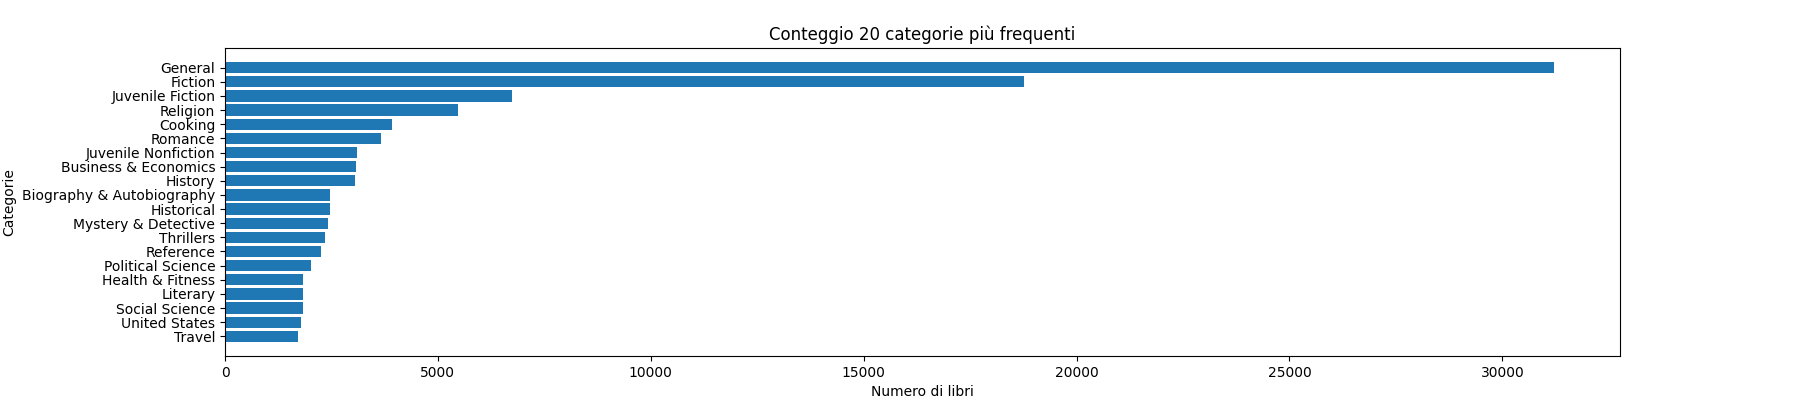
\includegraphics[width=0.96\textwidth]{pics/dati_iniziali.png}
    \begin{justify}
    Al seguente dataset più bilanciato:
    \end{justify}
    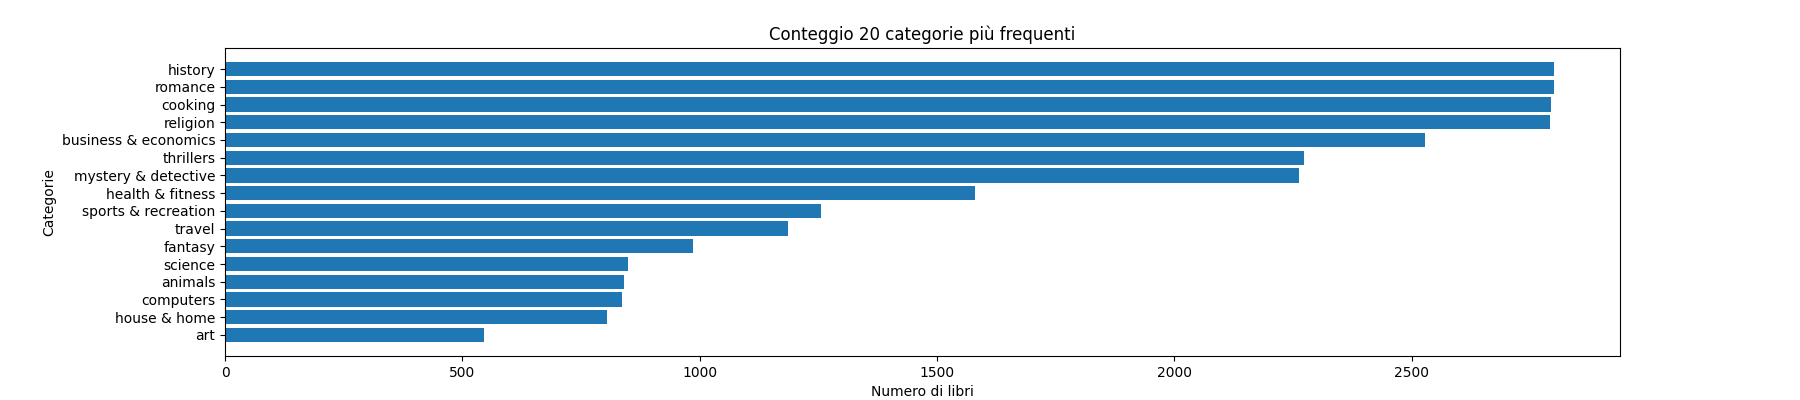
\includegraphics[width=0.96\textwidth]{pics/dati_postprocessati.png}

    \begin{minipage}[t]{0.40\textwidth}
    \vspace{30pt}
    Possiamo concludere che sono state effettuate le seguenti modifiche del dataset in questione, con la rimozione del seguente numero di righe:
    \end{minipage}
    \hfill
    \begin{minipage}[t]{0.50\textwidth}
    \vspace{20pt}
    \includegraphics[width=1\textwidth]{pics/bilanciamento.png}
    \end{minipage}
    \end{enumerate}

    \hfill
    \hfill
    \begin{enumerate}
    \subsection{Visualizzazione Word Cloud}
    \begin{justify}
    Grazie all'utilizzo delle WordCloud, nello specifico tramite l'utilizzo delle funzioni "createDescriptionWordCloud" e "createAuthorsWordCloud", è stato possibile illustrare le parole chiavi presenti all'interno delle descrizioni e degli autori. Verrano creati tanti WordCloud quante sono le categorie.
    \end{justify}
    \includegraphics[width=0.95\textwidth]{pics/descriptionWordCloud.png}
    
    \newpage
    \begin{justify}
    La seguente immagine è un esempio di output della funzione (con lo scopo di farne comprendere il corretto funzionamento, vengono mostrate solo quattro categorie):
    \end{justify}
    \begin{figure}[H]
    \centering
    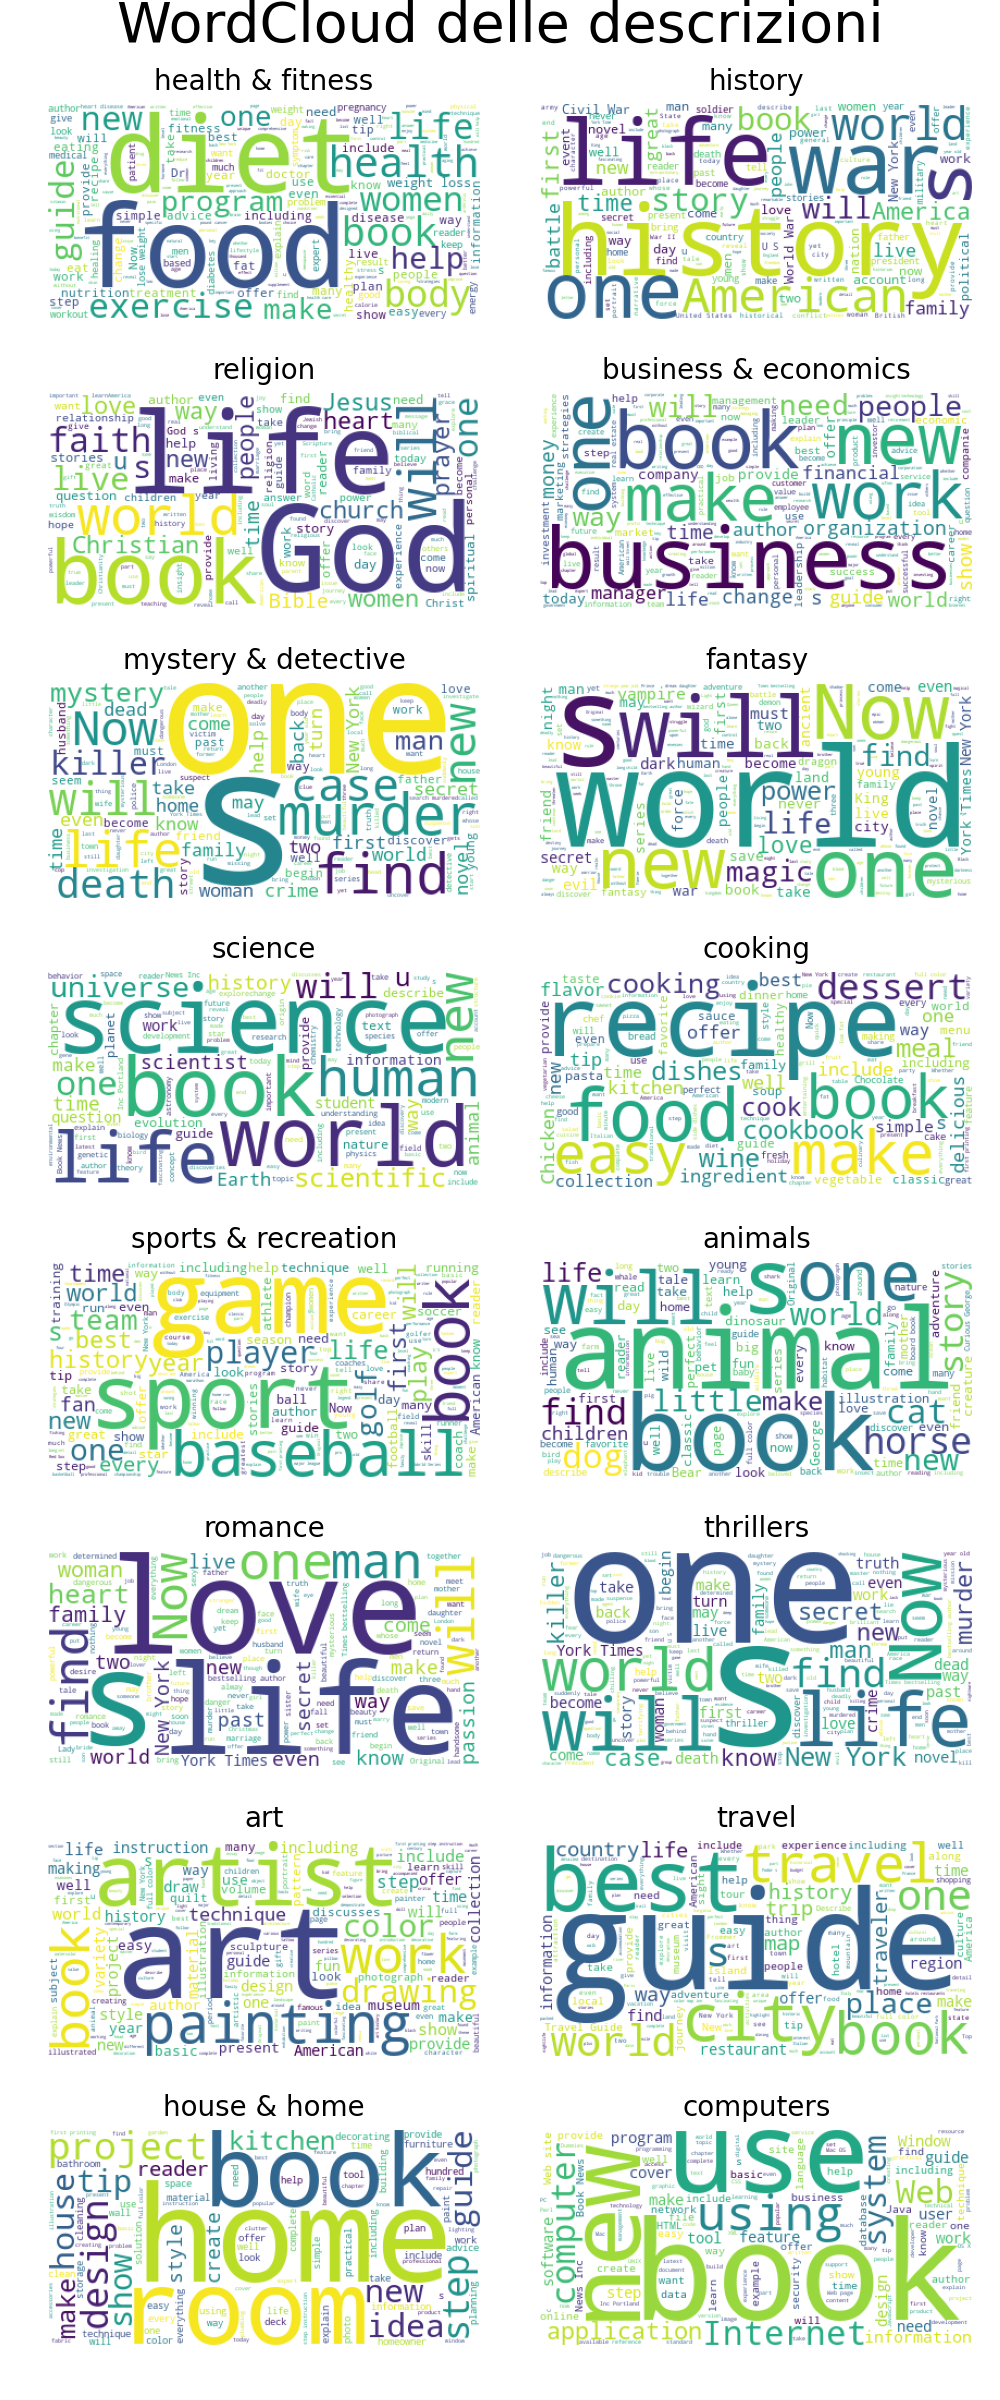
\includegraphics[width=0.90\textwidth]{pics/wordcloud_descrizioni_nonprocessate.png}
    \caption{Word Cloud delle descrizioni non processate}
    \end{figure}

    \hfill
    \begin{justify}
    Tale illustrazione ci permette di analizzare con più semplicità le parole ricorrenti ed individuare delle stop words aggiuntive, che fanno riferimento al dataset in questione, come ad esempio "book" e "life". Allo stesso ragionamento vengono sottoposti gli autori. Ecco le stop word individuate:
    \end{justify}
    \includegraphics[width=0.95\textwidth]{pics/aggiuntaStopWords.png}

    \newpage
    \begin{justify}
    Con la successiva eliminazione delle stop words individuate, si ottiene il seguente word cloud:
    \end{justify}
    \begin{figure}[H]
    \centering
    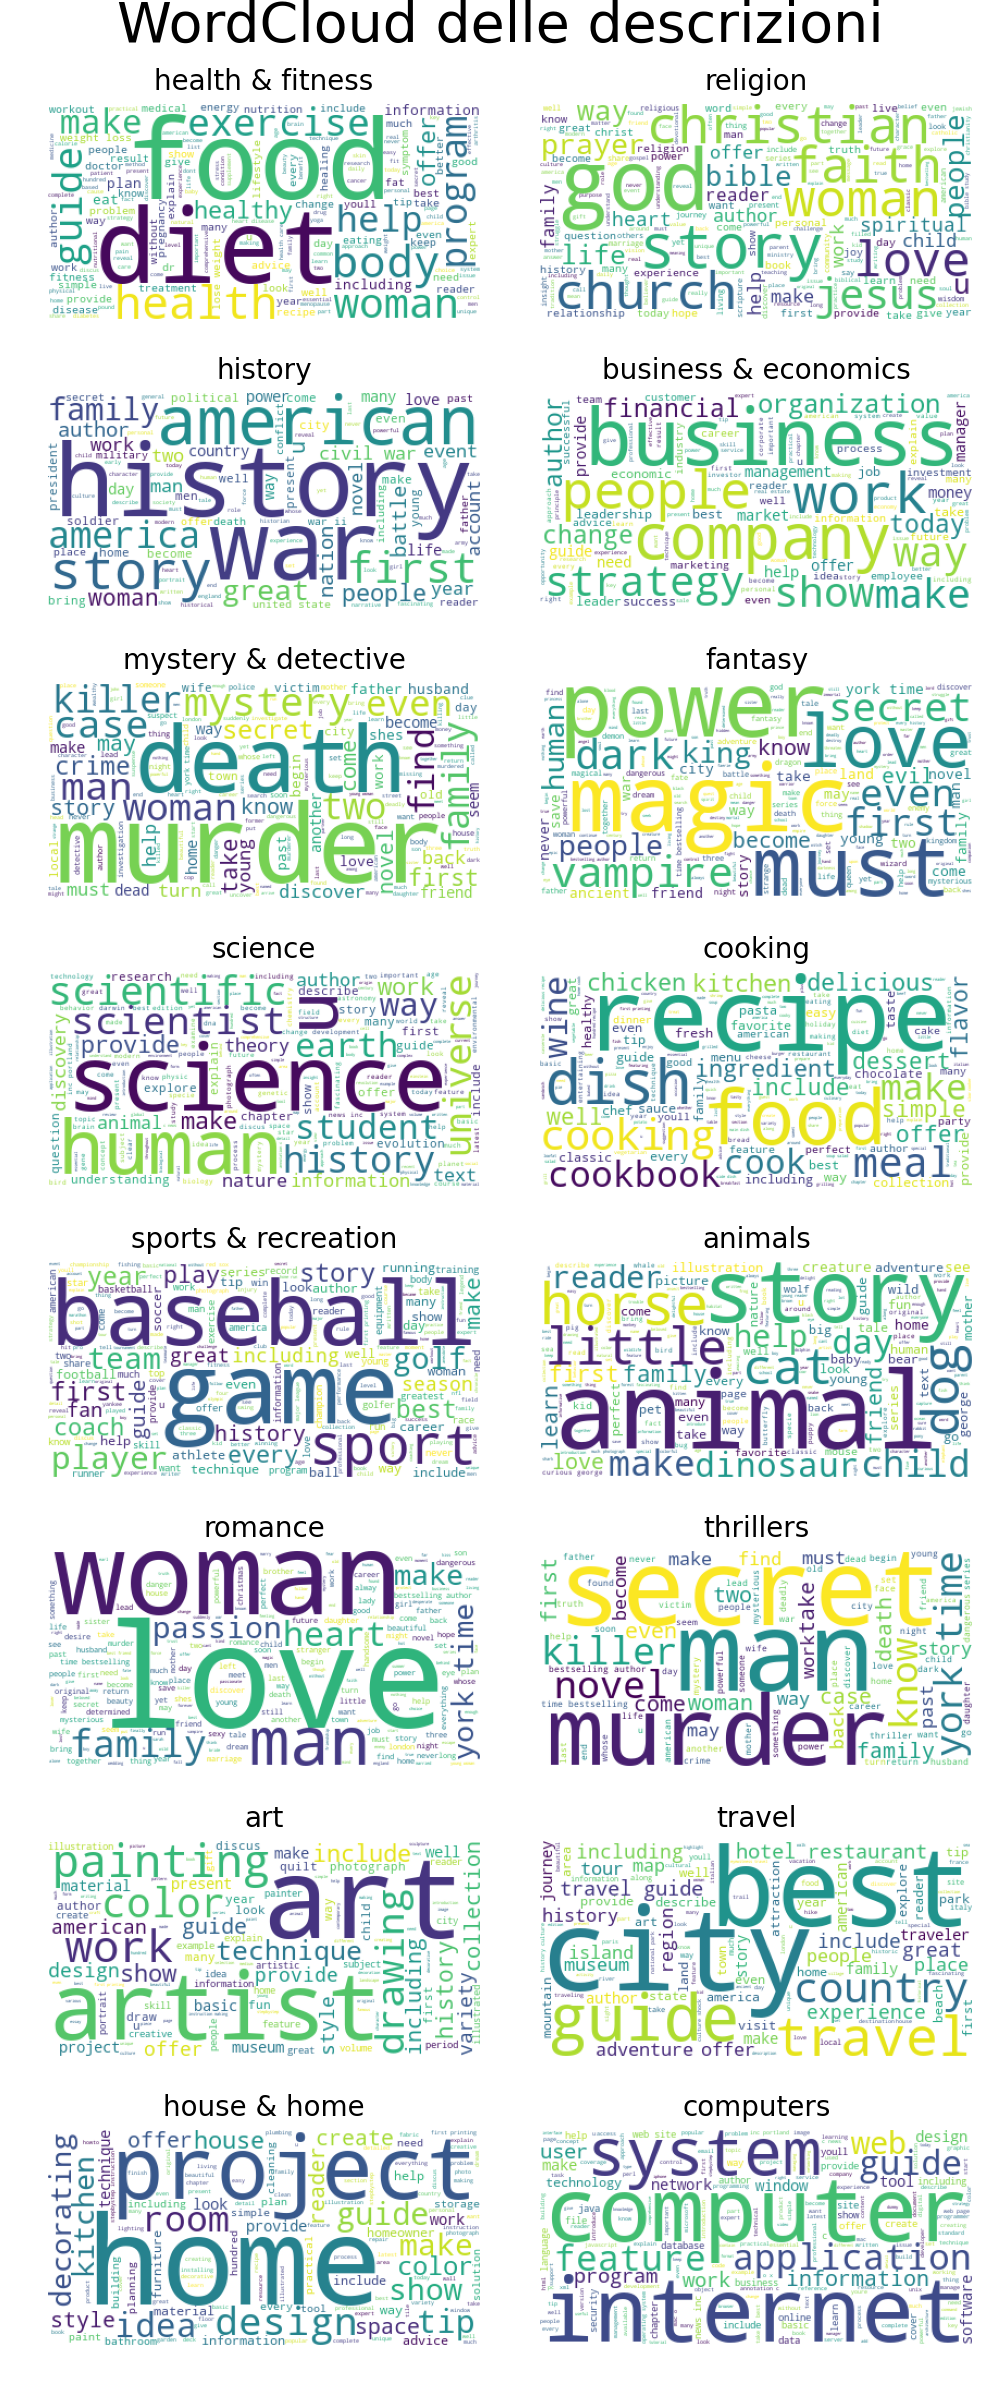
\includegraphics[width=0.95\textwidth]{pics/wordcloud_descrizioni_processate.png}
    \caption{Word Cloud delle descrizioni processate}
    \end{figure}

    \hfill
    \hfill
    \begin{figure}[H]
    \begin{subfigure}{0.48\textwidth}
    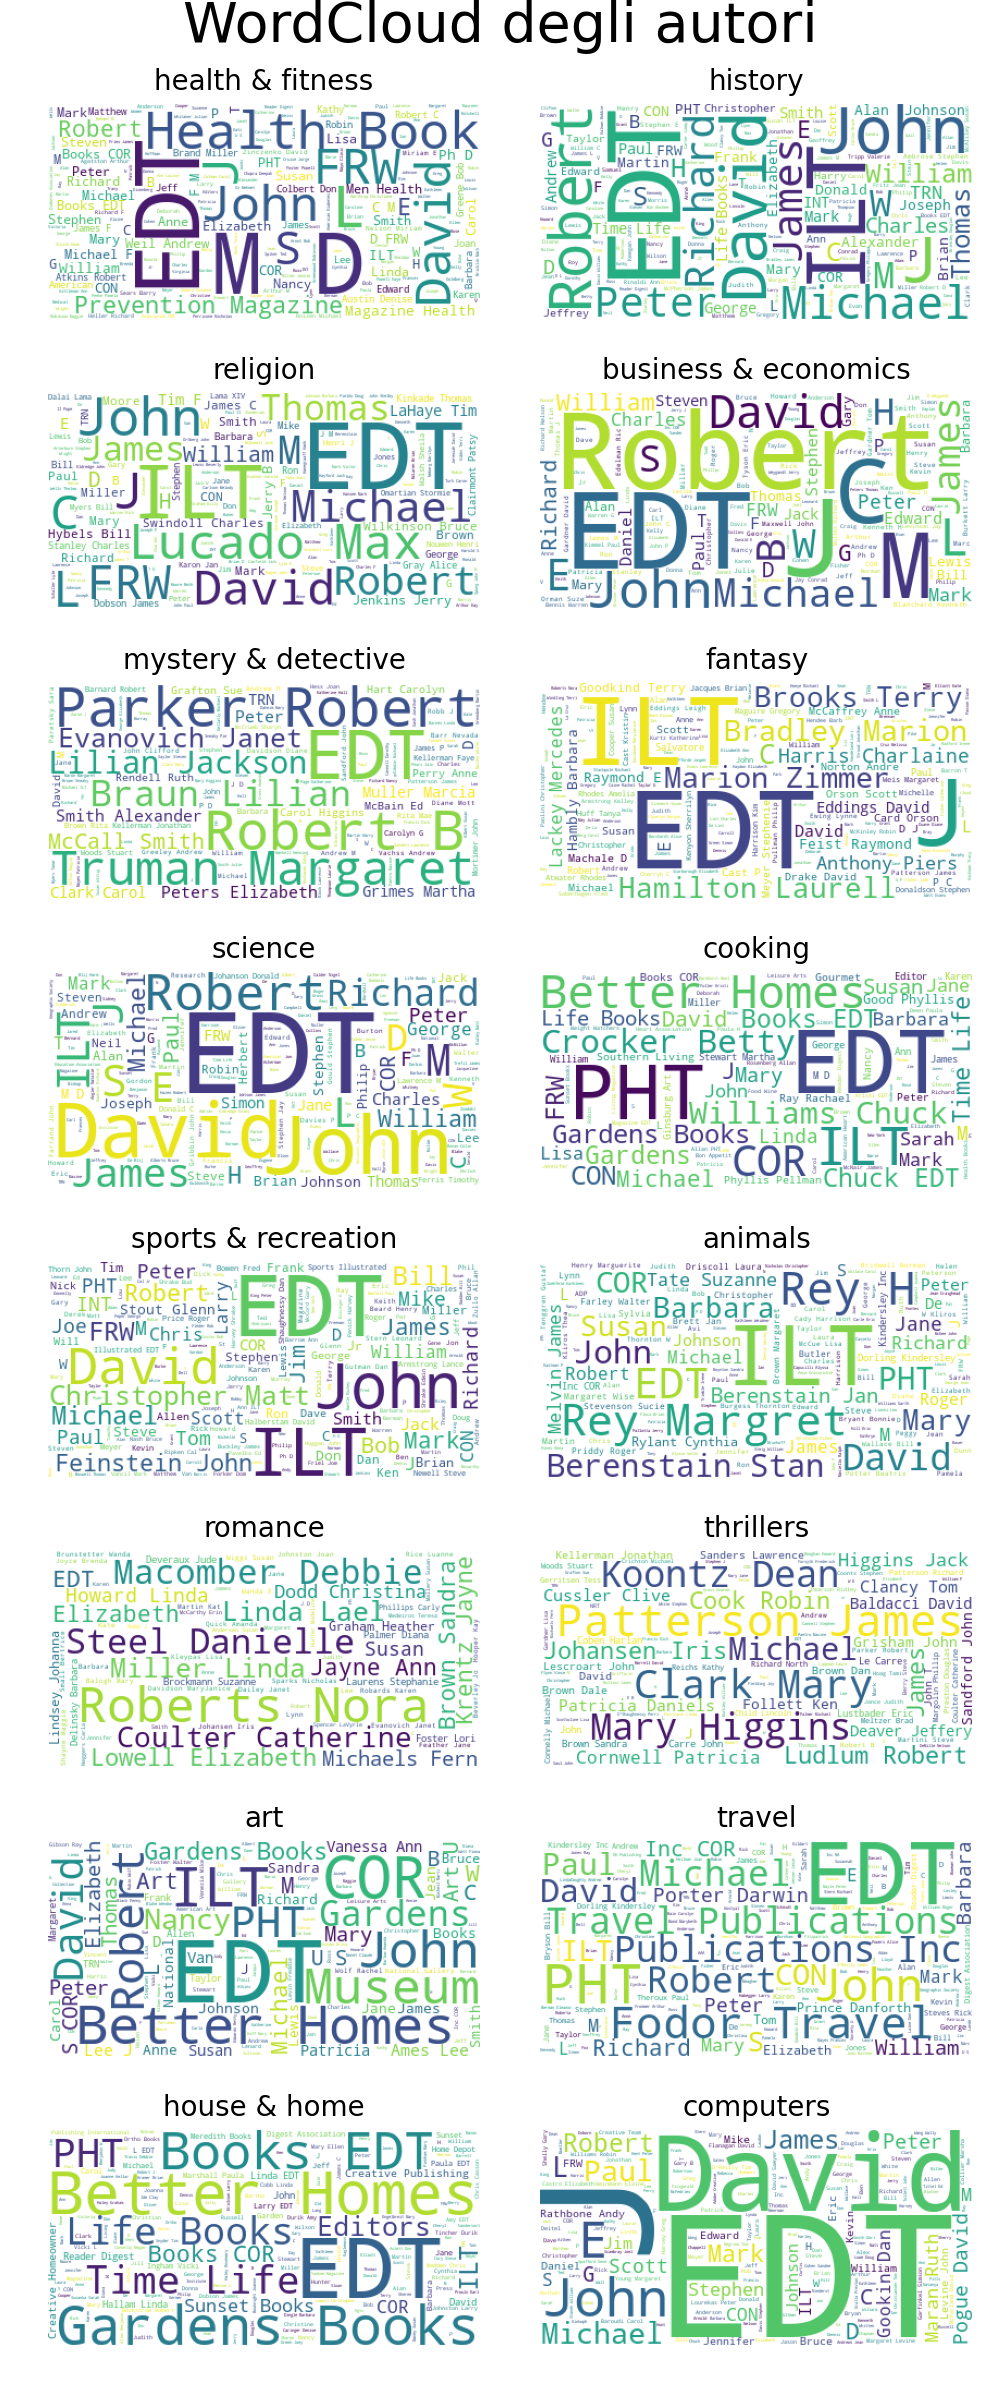
\includegraphics[width=\linewidth]{pics/wordcloud_autori_nonprocessati.png} 
    \caption{Word Cloud degli autori non processati}
    \label{fig:subim1}
    \end{subfigure}
    \begin{subfigure}{0.48\textwidth}
    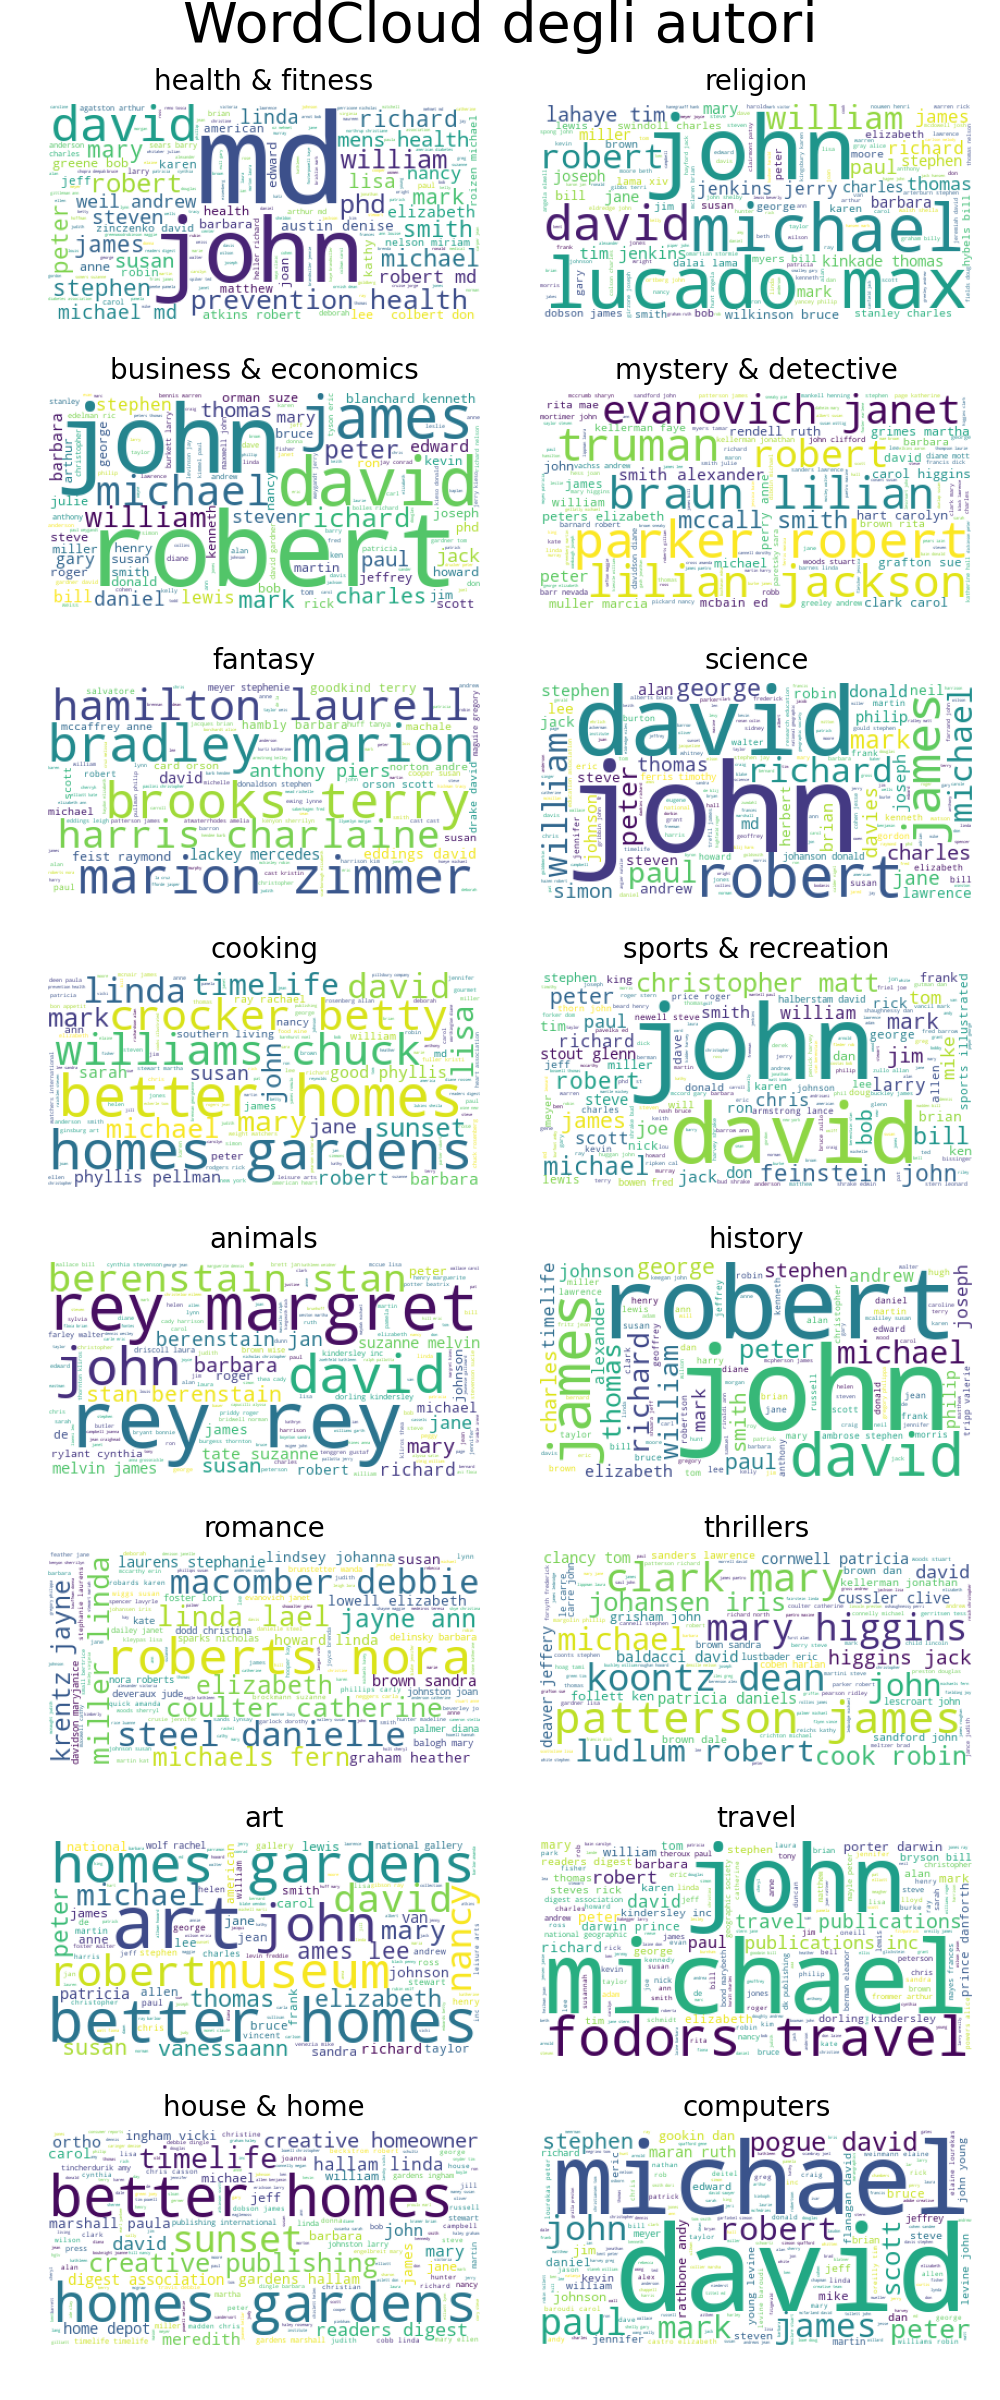
\includegraphics[width=\linewidth]{pics/wordcloud_autori_processati.png}
    \caption{Word Cloud degli autori processati}
    \label{fig:subim2}
    \end{subfigure}
    \caption{Word Cloud degli autori}
    \end{figure}
    \end{enumerate}



    \begin{enumerate}
    \subsection{Formattazione dei dati}
    \end{enumerate}


\section{Classificazione}
    \begin{enumerate}
    \subsection{Support Vector Classification}
    \end{enumerate}
   
    \begin{enumerate}
    \subsection{Mulinomial Classification}
    \end{enumerate}
    
    \begin{enumerate}
    \subsection{Logistic Classification}
    \end{enumerate}

    \begin{enumerate}
    \subsection{SGD Classification}
    \end{enumerate}
    
    \begin{enumerate}
    \subsection{Valutazione della Classificazione}
    \end{enumerate}


\section{Clustering}
    \begin{enumerate}
    \subsection{Algoritmo K-Means}
    \end{enumerate}

    \begin{enumerate}
    \subsection{Algoritmo MiniBatchKMean}
    \end{enumerate}

    \begin{enumerate}
    \subsection{Algoritmo SpectralClustering}
    \end{enumerate}

    \begin{enumerate}
    \subsection{Valutazione del Clustering: Silhouette score}
    \end{enumerate}

\section{Conclusioni}

    
\end{document}
